\documentclass[conference]{IEEEtran}
\IEEEoverridecommandlockouts
% The preceding line is only needed to identify funding in the first footnote. If that is unneeded, please comment it out.
%Template version as of 6/27/2024

\usepackage{cite}
\usepackage{amsmath,amssymb,amsfonts}
\usepackage{algorithmic}
\usepackage{graphicx}
\usepackage{textcomp}
\usepackage{xcolor}
\def\BibTeX{{\rm B\kern-.05em{\sc i\kern-.025em b}\kern-.08em
    T\kern-.1667em\lower.7ex\hbox{E}\kern-.125emX}}


%后加的包
\usepackage{booktabs}
\usepackage{multirow}
\usepackage[T1]{fontenc}
\usepackage{makecell}



\begin{document}
\bstctlcite{IEEEexample:BSTcontrol}
\title{Asteroid Inversion via ISAR Dynamic Envelope Consistency\\

\thanks{This work was supported by the National Natural Science Foundation of
	China under Grant 62227901.}
}

\author{\IEEEauthorblockN{1\textsuperscript{st} Zhicheng Xie}
\IEEEauthorblockA{\textit{School of Information and Electronics} \\
\textit{Beijing Institute of Technology}\\
Beijing, China \\
zhichengxieleo@163.com}
\and
\IEEEauthorblockN{2\textsuperscript{nd} Peiyao Liu}
\IEEEauthorblockA{\textit{School of Information and Electronics} \\
\textit{Beijing Institute of Technology}\\
Beijing, China \\
peiyao2429@163.com}
\and
\IEEEauthorblockN{3\textsuperscript{rd} Zhen Wang}
\IEEEauthorblockA{\textit{School of Information and Electronics} \\
\textit{Beijing Institute of Technology}\\
Beijing, China \\
wangzhenbit@163.com}
%\and
%\IEEEauthorblockN{4\textsuperscript{th} Zehua Dong}
%\IEEEauthorblockA{\textit{School of Information and Electronics} \\
%	\textit{Beijing Institute of Technology}\\
%	Beijing, China \\
%	z.dong@bit.edu.cn}
%\and
%\IEEEauthorblockN{5\textsuperscript{th} Zegang Ding}
%\IEEEauthorblockA{\textit{School of Information and Electronics} \\
%	\textit{Beijing Institute of Technology}\\
%	Beijing, China \\
%	z.ding@bit.edu.cn}
%\and
%\IEEEauthorblockN{6\textsuperscript{th} Given Name Surname}
%\IEEEauthorblockA{\textit{dept. name of organization (of Aff.)} \\
%	\textit{name of organization (of Aff.)}\\
%	City, Country \\
%	email address or ORCID}
}

\maketitle

\begin{abstract}
Accurate estimation of asteroid rotation and three-dimensional (3D) shape is critical for planetary defense, yet it remains challenging due to the geometric coupling between spin and shape and the lack of precise scale priors. This paper proposes a characterization framework featuring dynamic envelope consistency and two-stage dimensionality-reduced optimization. By matching the temporal evolution of Inverse Synthetic Aperture Radar (ISAR) dynamic envelopes and utilizing the Pearson Correlation Coefficient, the rotation dynamics are effectively decoupled from the absolute scale. Subsequently, the high-dimensional reconstruction is simplified into a stable 1D scalar search by constraining vertex displacements along analytical surface normals and incorporating signal-intensity-weighted Laplacian regularization. Computer simulation results validate the effectiveness of the proposed method.
\end{abstract}

\begin{IEEEkeywords}
asteroids, ISAR, rotation parameter estimation, 3D reconstruction, dynamic envelope consistency.
\end{IEEEkeywords}

\section{Introduction}

Asteroids are important non-cooperative targets in deep-space exploration and space surveillance. The accurate estimation of their rotation parameters and three-dimensional structures plays a critical role in planetary science studies, orbital evolution analysis, and planetary defense\cite{ostro2002a}.

Conventional observation approaches for asteroids mainly include optical telescopes and ground-based radar systems. Optical observations can provide photometric and contour information; however, they are highly sensitive to weather conditions and illumination geometry. In contrast, ground-based radar, as an active sensing modality, can acquire both range and Doppler information with high spatial resolution and strong geometric constraints\cite{benner2015}. In particular, inverse synthetic aperture radar (ISAR) imaging enables the reconstruction of two-dimensional scattering distributions of targets, providing a crucial data foundation for the estimation of rotation parameters and three-dimensional shape reconstruction.

In the feature inversion of asteroids, there exists a strong geometric coupling effect between rotation parameters and three-dimensional (3D) shape\cite{wang2023}. On the one hand, the joint estimation of both sets of parameters is severely ill-posed; the optimization process easily falls into local optima, triggering severe ambiguity and multi-solution problems. On the other hand, traditional separate estimation methods, when inverting rotation parameters such as pole orientation, are highly dependent on the absolute geometric scale of the target. An inaccurate initial scale prior often leads to severe estimation bias. Furthermore, directly optimizing high-dimensional 3D mesh vertices from 2D ISAR projections inevitably suffers from parameter explosion, making it highly susceptible to physical distortions such as mesh self-intersections and face flipping. 

To overcome the aforementioned challenges, this paper proposes a novel inversion framework featuring dynamic envelope consistency for rotation parameter estimation and two-stage dimensionality reduction for 3D shape reconstruction. The main contributions of this work are summarized as follows:

\begin{itemize}
	\item \textbf{Dynamic envelope consistency-based rotation estimation:} A scale-robust estimation strategy is developed by matching the temporal evolution trends of ISAR dynamic envelopes. By utilizing the Pearson Correlation Coefficient (PCC) to quantify the similarity of geometric trajectories and incorporating a symmetry-compensated cosine distance for tilt angles, this approach effectively decouples the rotation dynamics from the absolute dimensions of the target while resolving the $180^\circ$ geometric ambiguity.
	
	\item \textbf{Normal-constrained two-stage shape inversion:} A dimensionality-reduction optimization framework is proposed to transform the high-dimensional 3D mesh refinement into a 1D scalar displacement problem along analytical surface normals. By incorporating a spatial-adaptive Laplacian regularization weighted by local signal intensity, the approach effectively suppresses reconstruction artifacts in low-SNR regions while preserving fine shape details.
\end{itemize}

The remainder of this paper is organized as follows. Section \ref{sec_two} establishes the ground-based radar observation geometry and the ISAR echo signal model. Section \ref{sec_three} details the proposed rotation parameter estimation strategy and the two-stage 3D shape reconstruction algorithm. Section \ref{sec_four} presents comprehensive computer simulations and quantitative evaluations based on the high-precision 3D model of asteroid 1999~JV6 and the flyby ephemeris of 1999~AN10. Finally, Section \ref{sec_five} concludes the paper.

\section{Ground-Based Radar Observation Geometry and Signal Model}\label{sec_two}


\subsection{Observation Geometry}\label{Observation}

Due to the combined effects of self-gravity, rotation, and long-term collisional evolution, the global shape of most asteroids can be approximated as a triaxial ellipsoid\cite{campbell2002}, which is adopted in this paper as the initial geometric baseline for 3D reconstruction.

First, an asteroid intrinsic coordinate system, denoted as $O-xyz$, is established with its origin at the target's center of mass. The $x$-axis aligns with the ellipsoid's major axis (with a semi-axis length of $a$), while the $y$- and $z$-axes are orthogonally determined by the right-hand rule (with semi-axis lengths of $b$ and $c$, respectively). Within this intrinsic coordinate system, the 3D geometric morphology of the initial reference ellipsoid is uniquely characterized by the shape covariance matrix $\mathbf{\Sigma}_0 = \text{diag}(a^2, b^2, c^2)$.

Most asteroids can be regarded as freely rotating rigid bodies without external torques. Assuming simple rotation about the principal axis of inertia (which aligns with the $z$-axis of the intrinsic coordinate system), the spin period $T$ and the pole direction remain constant during the observation. Let the scalar angular velocity be $\omega = 2\pi/T$, yielding the angular velocity vector $\boldsymbol{\omega} = [0, 0, \omega]^T$. The pole direction is uniquely determined by the ecliptic longitude $\lambda$ and ecliptic latitude $\beta$. To establish the observation geometry, the ecliptic coordinate system is mapped to the asteroid intrinsic coordinate system, as illustrated in Fig. \ref{fig_coordinate}.

\begin{figure}[htbp]
	\centerline{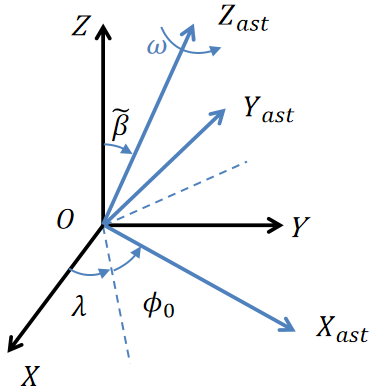
\includegraphics[width=0.4\columnwidth]{fig_coordinate.png}}
	\caption{Ecliptic to asteroid intrinsic coordinate transformation.}
	\label{fig_coordinate}
\end{figure}

Let $\mathbf{P}_{ecl}(t)$ denote the radar position vector in the ecliptic frame, obtained from the Jet Propulsion Laboratory (JPL) Horizons system. Through successive Euler angle rotations based on $\lambda$, $\beta$, and the initial observation phase $\phi_0$, its coordinates in the asteroid intrinsic coordinate system, denoted as $\mathbf{P}_{ast}(t)$, can be calculated via \cite{Gao2026}:
\begin{equation}
	\mathbf{P}_{ast}(t) = \mathbf{R}_z(\omega t + \phi_0) \mathbf{R}_y(\widetilde{\beta}) \mathbf{R}_z(\lambda) \cdot \mathbf{P}_{ecl}(t)
\end{equation}
where $\widetilde{\beta} = 90^\circ - \beta$ represents the ecliptic co-latitude, and $\mathbf{R}_z(\cdot)$ and $\mathbf{R}_y(\cdot)$ denote the passive coordinate rotation matrices around the $z$-axis and $y$-axis, respectively.

Finally, let $\mathbf{u}_{r}(t)$ be the unit line-of-sight (LOS) vector pointing from the asteroid's center of mass toward the radar in the intrinsic coordinate system, which is defined as $\mathbf{u}_{r}(t) = \mathbf{P}_{ast}(t) / \|\mathbf{P}_{ast}(t)\|= \big[ u_x(t), u_y(t), u_z(t) \big]^T$. 

Notably, under the far-field assumption for ground-based radar observations of asteroids, the incident wave can be approximated as a plane wave, implying that the unit LOS vector $\mathbf{u}_{r}(t)$ remains spatially identical across the entire target body. This time-varying unit vector characterizes the dynamic observation perspective and serves as the fundamental projection axis for the subsequent radar echo modeling and 3D reconstruction.

\subsection{Echo Signal Model and Image Formation}\label{Echo}

For an asteroid rotating as a rigid body, the ground-based radar echo is modeled as the coherent summation of reflections from all visible surface scattering points. Assuming the macroscopic translational bulk motion $R_0(t)$ of the asteroid's center of mass has been fully compensated via standard envelope alignment and dechirp processing of the Wideband Linear Frequency Modulated (LFM) signals, the final focused ISAR image $I(f_d, r)$ in the range-Doppler domain can be analytically formulated as the superposition of 2D Point Spread Function (PSF) responses\cite{busch2010}\cite{brozovic2009}:
\begin{equation}
	I(f_d, r) = \sum_{i \in \mathbb{V}} \sigma_i \cdot h \left( f_d - f_{di}, r - r_i \right)
\end{equation}
where $\mathbb{V}$ denotes the set of all visible scattering points considering self-occlusion, and $\sigma_i$ is the backscattering coefficient of the $i$-th point, given by $\sigma_i \propto \cos^2\theta_i$, with $\theta_i$ being the local incidence angle\cite{zhou2023}. The function $h(\cdot, \cdot)$ represents the 2D radar PSF, whose mainlobe dimensions are determined by the theoretical Doppler resolution $\rho_d = 1 / T_{obs}$ and range resolution $\rho_r = c / (2B)$, with $c$ being the speed of light, $T_{obs}$ the coherent integration time, and $B$ the signal bandwidth.

Geometrically, the ideal 2D projection coordinates $(f_{di}, r_i)$ of the $i$-th scatterer at 3D position $\mathbf{r}_i$ are mapped via:
\begin{equation}
	\begin{cases}
		f_{di}(t) = \frac{2}{\lambda_{wav}} \langle \mathbf{u}_r(t) \times \boldsymbol{\omega}, \mathbf{r}_i \rangle \\
		r_i(t) = \langle \mathbf{u}_r(t), \mathbf{r}_i \rangle
	\end{cases}
	\label{fdi_ri}
\end{equation}
where $\lambda_{wav}$ is the radar wavelength.

Rewriting this point-to-pixel mapping in a compact matrix form, we define the $2 \times 3$ linear projection matrix $\mathbf{H}(t)$:
\begin{equation}
	\mathbf{H}(t) = 
	\begin{bmatrix}
		\frac{2}{\lambda_{wav}} \left( \mathbf{u}_r(t) \times \boldsymbol{\omega} \right)^T \\
		\mathbf{u}_r^T(t)
	\end{bmatrix}
\end{equation}

Consequently, for a triaxial asteroid characterized by the initial 3D shape covariance matrix $\mathbf{\Sigma}_0$, its global theoretical envelope in the 2D ISAR image is strictly the affine transformation of $\mathbf{\Sigma}_0$ under $\mathbf{H}(t)$. The projected 2D covariance matrix $\mathbf{\Sigma}_{RD}(t)$ characterizing the global ISAR contour is directly derived as:
\begin{equation}
	\mathbf{\Sigma}_{RD}(t) = \mathbf{H}(t)\,\mathbf{\Sigma}_0\,\mathbf{H}^T(t) =
	\begin{bmatrix}
		c_{11}(t) & c_{12}(t) \\
		c_{12}(t) & c_{22}(t)
	\end{bmatrix}
\end{equation}
%where
%\begin{equation}
%	\begin{cases}
%		c_{11}(t) = \left( \frac{4\pi}{\lambda_{wav} T} \right)^2 \left( a^2 u_y^2(t) + b^2 u_x^2(t) \right) \\
%		c_{12}(t) = c_{21}(t) = \frac{4\pi}{\lambda_{wav} T} u_x(t) u_y(t) \left( a^2 - b^2 \right) \\
%		c_{22}(t) = a^2 u_x^2(t) + b^2 u_y^2(t) + c^2 u_z^2(t)
%	\end{cases}
%\end{equation}

By directly extracting the elements of $\mathbf{\Sigma}_{RD}(t)$, the tangible macroscopic geometric features of the envelope on the Range-Doppler plane can be analytically formulated. Specifically, the theoretical Doppler width $\hat{L}_{d}(t)$, the range length $\hat{L}_{r}(t)$, and the tilt angle $\hat{\theta}(t)$ of the ISAR envelope relative to the Doppler frequency domain are strictly determined by the matrix elements as follows:
\begin{equation}
	\begin{cases}
		\hat{L}_{d}(t) = 2\sqrt{c_{11}(t)} \\
		\hat{L}_{r}(t) = 2\sqrt{c_{22}(t)} \\
		\hat{\theta}(t) = \frac{1}{2} \arctan \left( \frac{2 c_{12}(t)}{c_{11}(t) - c_{22}(t)} \right)
	\end{cases}
\end{equation}

\section{Proposed Method}\label{sec_three}

%In this section, 


\subsection{Rotation Parameter Estimation}\label{Rotation}

To address the challenge of inaccurate scale priors for non-cooperative targets, a rotation parameter estimation strategy based on dynamic envelope consistency is proposed. By matching the temporal evolution trends of geometric features, this approach effectively decouples the rotation parameters $\Omega = \{T, \phi_0, \lambda, \beta\}$ from the absolute dimensions of the target.

In practical ISAR observations, the theoretical macroscopic features cannot be directly obtained due to the inevitable LOS self-occlusion effect. Therefore, to ensure unbiased parameter estimation, the actual geometric features must be extracted from the partially occluded 2D images and directly evaluated against features extracted under the identical simulation pipeline.

Specifically, assume that a sequence of $N$ ISAR images is obtained at discrete observation times $\{t_k\}_{k=1}^N$. The target region is extracted via morphological processing, from which the second-order central moments are computed to derive the observed envelope tilt angle sequence $\boldsymbol{\theta} = \{\theta(t_k)\}_{k=1}^N$. Concurrently, by projecting valid pixels onto the Doppler and range axes, the Doppler width sequence $\mathbf{L}_d = \{L_d(t_k)\}_{k=1}^N$ and range length sequence $\mathbf{L}_r = \{L_r(t_k)\}_{k=1}^N$ are obtained.

The rotation parameters are estimated via a scale-invariant cost function $J(\Omega)$. For the tilt angle sequence, the cosine distance is employed to measure the temporal discrepancy, where a factor of 2 resolves the $180^\circ$ ambiguity inherent in geometric symmetry. For the Doppler width and range length sequences, the PCC is utilized to quantify the similarity of their temporal evolution trends. This formulation explicitly decouples the rotation parameters from the absolute geometric scale based on temporal dynamics.

The final cost function is formulated as:
\begin{equation}
	\begin{split}
		J(\Omega) &= w_1 \left( 1 - \frac{1}{N} \sum_{k=1}^N \cos \Big( 2 \big( \theta(t_k) - \hat{\theta}(t_k; \Omega) \big) \Big) \right) \\
		&\quad + w_2 \big( 1 - \text{Corr}(\mathbf{L}_d, \hat{\mathbf{L}}_d(\Omega)) \big) \\
		&\quad + w_3 \big( 1 - \text{Corr}(\mathbf{L}_r, \hat{\mathbf{L}}_r(\Omega)) \big)
	\end{split}
\end{equation}
where $\hat{\theta}(t_k; \Omega)$, $\hat{\mathbf{L}}_d(\Omega)$, and $\hat{\mathbf{L}}_r(\Omega)$ denote the theoretical sequences predicted by the parameter set $\Omega$; $\text{Corr}(\cdot, \cdot)$ denotes the Pearson correlation operator, and $w_1, w_2, w_3$ are weighting coefficients. Considering that the self-occlusion effect along the LOS attenuates the reliability of range length observations, $w_3$ is typically assigned a smaller value compared to $w_1$ and $w_2$.

Due to the highly non-linear and multi-modal nature of $J(\Omega)$, gradient-based methods are prone to local optima. Consequently, a Genetic Algorithm (GA) is employed to explore the non-convex search space and identify the global optimum.  

\subsection{Shape Parameter Inversion}\label{Shape}

Based on the estimated rotation parameters $\Omega$, 3D shape inversion is performed to recover the geometric scale and fine topography. Direct optimization of a high-dimensional 3D mesh from 2D projections is ill-posed. To address this, a two-stage decoupled optimization framework is adopted.

\subsubsection{Stage 1}

The global shape is approximated by a tri-axial ellipsoid with scale factors $\mathbf{s} = [a, b, c]$. The optimal $\mathbf{s}$ is estimated by minimizing the normalized amplitude residual between simulated and observed ISAR images\cite{brozovic2010}:
\begin{equation}
	\mathbf{s}^* = \arg\min_{\mathbf{s}} \frac{1}{N_{pix}} \sum \left( \frac{\hat{I}_{sim}(\mathbf{s}; \Omega) - I_{obs}}{\sigma_{noise}} \right)^2
\end{equation}
where $N_{pix}$ is the total number of pixels, $I_{obs}$ and $\hat{I}_{sim}$ denote the observed and simulated amplitudes, and $\sigma_{noise}$ is the noise standard deviation.

\subsubsection{Stage 2}

In the second stage, local geometric details are refined by constraining vertex displacements along the analytical surface normals $\mathbf{N}_{base}$. The updated shape is expressed as
\begin{equation}
	\mathbf{V}_{opt} = \mathbf{V}_{base} + \Delta \mathbf{r} \odot \mathbf{N}_{base}
\end{equation}

where $\Delta \mathbf{r}$ denotes the scalar displacement along the normal direction.

Compared with directly optimizing full 3D vertex coordinates, this formulation reduces the dimensionality of the solution space and improves optimization stability, while avoiding mesh distortions such as face flipping and self-intersections.

The displacement is estimated by minimizing the following objective function:
\begin{equation}
	J_{micro}(\Delta \mathbf{r}) = E_{data}(\Delta \mathbf{r}) + \lambda E_{lap}(\Delta \mathbf{r}, \mathbf{W})
\end{equation}

where $E_{data}$ is the data fidelity term derived from amplitude residuals, and $E_{lap}$ is a Laplacian regularization term. The spatial weight $\mathbf{W}$ is defined as
\begin{equation}
	W^{(i)} = \frac{\epsilon}{\rho^{(i)} + \epsilon}
\end{equation}
where $\epsilon$ is a small constant and $\rho^{(i)}$ is a normalized cumulative signal intensity. This weighting strategy effectively enforces stronger smoothness constraints on low-SNR regions to suppress reconstruction artifacts while allowing high-energy regions to preserve fine geometric details. The parameter $\lambda$ balances data fidelity and smoothness.

To further reconstruct finer surface details, a hierarchical refinement strategy is incorporated into this stage. Upon convergence of the vertex displacement optimization on the initial coarse mesh, Loop subdivision is applied to expand the geometric degrees of freedom, enabling the mesh to fit the target's continuous true shape more closely. The aforementioned normal-constrained optimization is subsequently re-executed on the subdivided higher-resolution surface.
\section{Simulation Experiments}\label{sec_four}

%In this section, computer simulation experiments are conducted to validate the aforementioned analysis and demonstrate the effectiveness of the proposed method.

\subsection{Simulation Setup}

A realistic 3D mesh model of asteroid 1999~JV6\cite{rozek2019}, obtained from the \textit{3D Asteroid Catalogue}, is utilized as the ground truth in our simulations. The model is scaled to dimensions of 44.39~m, 21.92~m, and 20.88~m along the X, Y, and Z axes, respectively. The corresponding coordinate ranges are defined as $x \in [-22.37, 22.02]$~m, $y \in [-11.71, 10.21]$~m, and $z \in [-10.85, 10.03]$~m.

The ground-based radar operates in the X-band with a center frequency of 9.6~GHz. To accommodate the asteroid's scale, the system bandwidth is set to 150~MHz, yielding a range resolution of 1~m. The coherent integration time for each ISAR frame is 100~s, corresponding to a Doppler resolution of 0.01~Hz.

The asteroid rotation parameters are configured as follows: the spin period is 9.0~h (32,400~s). The rotation axis orientation is specified in the ecliptic coordinate system with longitude $\lambda=23.3^{\circ}$ and latitude $\beta=45.0^{\circ}$. The initial rotation phase is set to $\phi_0=60.0^{\circ}$.

To account for realistic radar receiver characteristics, a noise model is incorporated into the simulated ISAR intensity images. A constant additive thermal noise floor is globally injected across all observation epochs to simulate a realistic ground-based radar system. The noise power is calibrated such that the peak signal-to-noise ratio (SNR) across the entire observation sequence is 8~dB.

To simulate a realistic observation trajectory, the time-varying geometry is derived from the 2027 flyby ephemeris of asteroid 1999~AN10. A total of 18 ISAR frames are generated over two distinct observation epochs: $t \in [0, 8]$~h and $t \in [59.2, 67.2]$~h. Each epoch provides 9 uniformly sampled frames at 1-hour intervals. This dual-epoch scheme ensures sufficient geometric diversity to mitigate self-occlusion effects. To intuitively illustrate this, the corresponding radar LOS directions in the asteroid intrinsic coordinate system are plotted in Fig.~\ref{fig_radar_los}. The simulation parameters are summarized in Table~\ref{tab_sim_params}.

\begin{figure}[htbp]
	\centerline{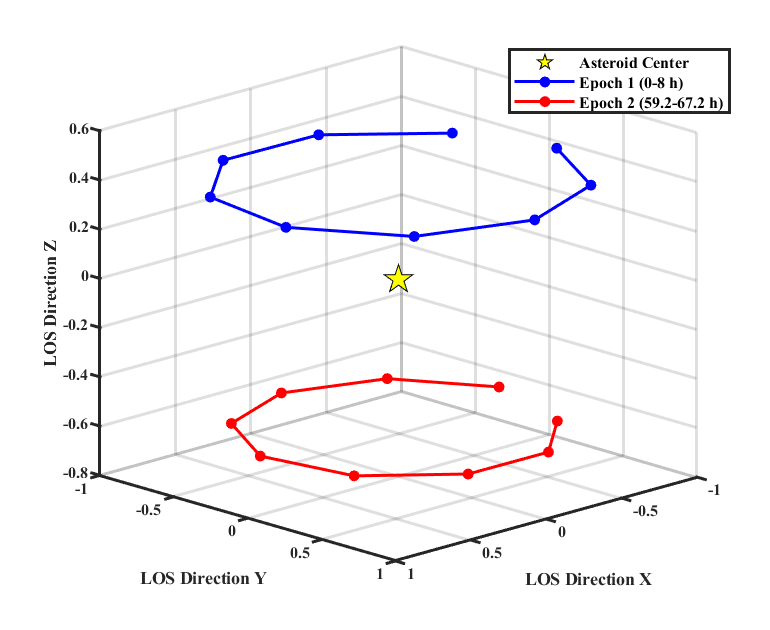
\includegraphics[width=0.6\columnwidth]{fig_radar_los.png}}
	\caption{Radar LOS directions in the asteroid intrinsic coordinate system across two observation epochs.}
	\label{fig_radar_los}
\end{figure}

\begin{table}[htbp]
	\caption{Key Parameters of the ISAR Simulation}
	\label{tab_sim_params}
	\centering
	% 1. 稍微拉大行距，给数据足够的“呼吸空间”
	\renewcommand{\arraystretch}{1.25} 
	\begin{tabular}{clcc} 
		\toprule % 2. 使用 booktabs 的加粗顶线
		\textbf{Category} & \textbf{Parameter} & \textbf{Symbol} & \textbf{Value} \\ 
		\midrule % 3. 使用较细的分隔线
		
		% 4. 使用 makecell 让类别名称优雅换行且居中
		\multirow{4}{*}{\makecell{Target \\ (1999 JV6)}} 
		& Dimensions & ($X, Y, Z$) & 44.39, 21.92, 20.88~m \\ 
		& Spin period & $T$ & 9.0~h \\ 
		& Rotation axis & ($\lambda, \beta$) & $23.3^\circ, 45.0^\circ$ \\ 
		& Initial phase & $\phi_0$ & $60.0^\circ$ \\ 
		\midrule % 类别之间的分隔线
		
		\multirow{4}{*}{\makecell{Radar \\ System}} 
		& Carrier frequency & $f_c$ & 9.6~GHz \\ 
		& Bandwidth & $B$ & 150~MHz \\ 
		& Range resolution & $\rho_r$ & 1~m \\ 
		& Doppler resolution & $\rho_d$ & 0.01~Hz \\ 
		\midrule % 类别之间的分隔线
		
		\multirow{3}{*}{Observation} 
		& Observation epochs & $N_{ep}$ & 2 \\ 
		& Total frames & $N_{fr}$ & 18 \\ 
		& SNR & $\mathit{SNR}$ & 8~dB \\ 
		\bottomrule % 5. 使用 booktabs 的加粗底线收尾
	\end{tabular}
\end{table}

\subsection{Rotation Parameter Estimation Results}

Based on the ISAR image envelopes, the dimensions of the reference triaxial ellipsoid are pre-estimated as $a=20$~m, $b=10$~m, and $c=10$~m. With this geometric baseline established, directly performing a single global blind search across the vast 4D kinematic parameter space is highly susceptible to local minima under severe noise interference. Therefore, we adopt a practical iterative range-narrowing search strategy. By conducting multiple independent iterations with progressively narrowed search bounds for the spin period $T$, a representative optimal solution that minimizes the proposed envelope-based cost function is identified, as summarized in Table~\ref{tab_estimation_results}.

\begin{table}[htbp]
	\caption{Comparison of True and Initially Estimated Rotation Parameters}
	\label{tab_estimation_results}
	\centering
	\renewcommand{\arraystretch}{1.25} % 与上一张表保持相同的行高比例
	\setlength{\tabcolsep}{6pt}      % booktabs自带留白，列间距可以稍微放宽一点
	\begin{tabular}{cccccc}
		\toprule % 顶部粗线
		\textbf{Symbol} & \textbf{Bounds} & \textbf{Initial} & \textbf{Truth} & \textbf{Estimated} & \textbf{Fixed $T$} \\ 
		\midrule % 细中线
		$T$ (h) & $[8.0, 12.0]$ & 8.00 & 9.00 & 8.979 & \textbf{9.000} \\ 
		$\lambda$ ($^{\circ}$) & $[0, 360]$ & 0.0 & 23.3 & 31.170 & \textbf{21.687} \\ 
		$\beta$ ($^{\circ}$) & $[-90, 90]$ & 0.0 & 45.0 & 60.024 & \textbf{44.375} \\ 
		$\phi_0$ ($^{\circ}$) & $[0, 180]$ & 0.0 & 60.0 & 58.351 & \textbf{59.688} \\ 
		\bottomrule % 底部粗线
	\end{tabular}
\end{table}

As shown in Table~\ref{tab_estimation_results}, the radar-only algorithm accurately captures the spin period $T$ and initial phase $\phi_0$ with minor errors (e.g., $\Delta T \approx 0.02$~h), demonstrating its robustness in locking onto the rotational rhythm. However, a noticeable deviation of approximately $15^{\circ}$ is observed in the pole latitude $\beta$ ($60.0^{\circ}$ vs. $45.0^{\circ}$). This significant spatial pose deviation fundamentally stems from the \textit{spatio-temporal coupling effect} within the rotation matrix. Due to the extensive 59.2-hour observation gap, the micro-error in $T$ (0.02~h) is amplified by a ``temporal lever'' into a severe cumulative phase drift. To minimize the matching error of the projected silhouettes in the later observation epoch, the optimizer is forced to substantially distort the pole direction ($\lambda, \beta$), artificially compensating for the phase misalignment on the time axis through a change in spatial perspective.

To break this ill-posed spatio-temporal coupling, an optical lightcurve prior ($T = 9.00$~h) is introduced in the ``Fixed $T$'' column. As shown in Table~\ref{tab_estimation_results}, once the temporal phase drift is entirely eliminated, the algorithm successfully escapes the massive compensatory trap, significantly reducing the spatial pose errors. At this stage, the residual minor pose deviation transitions into a typical \textit{modeling compensation} phenomenon---the optimizer fine-tunes the ellipsoid's perspective to bridge the morphological mismatch between the symmetric ellipsoid and the asymmetric micro-features of the actual asteroid. This fixed-$T$ configuration provides a highly robust topological initialization for the subsequent 3D shape deformation. Furthermore, the residual ``structural gap'' between the ellipsoid projections and the actual silhouettes provides the necessary gradient information to drive the upcoming shape reconstruction.

To qualitatively evaluate the final kinematic estimation, the simulated 2D ISAR projections based on the prior-constrained parameters are compared with the ground truth in Fig.~\ref{fig_disp_full_width}. The rotation rhythm and orientation of the simulated envelopes are highly consistent with the observations, validating the estimated kinematic parameters.

\begin{figure*}[htbp]
	\centering
	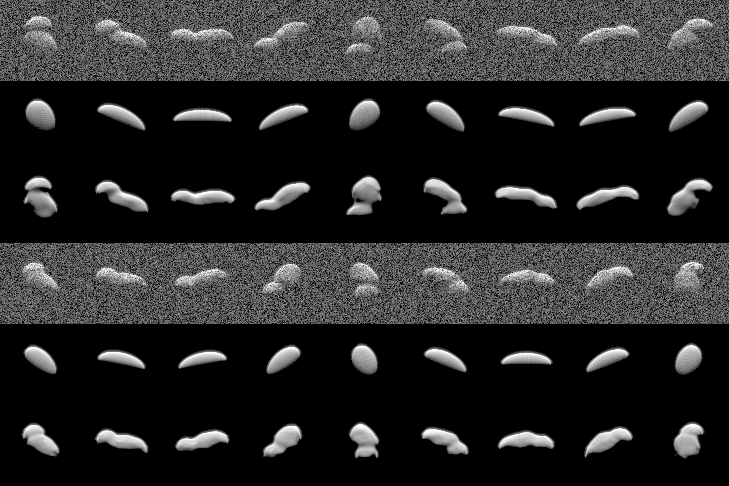
\includegraphics[width=0.8\textwidth]{imgResult_shape2026-04-16-15-58.png}
	\caption{Comparison of observed and simulated ISAR images (54 frames in total). Rows 1 and 4 display the ground truth ISAR projections for Epoch 1 (Frames 1--9) and Epoch 2 (Frames 10--18), respectively. Rows 2 and 5 show the corresponding simulations of the initial ellipsoid model using the prior-constrained rotation parameters. Rows 3 and 6 present the simulated ISAR projections of the final reconstructed 3D model.}
	\label{fig_disp_full_width}
\end{figure*}


\subsection{Shape Parameter Inversion Results}
Building upon the robust kinematic initialization provided by the prior-constrained rotation parameters, a two-stage shape parameter inversion is executed to reconstruct the fine 3D shape of asteroid 1999~JV6.

In the first stage, the global scale factors $\mathbf{s} = [a, b, c]$ are optimized to minimize the global envelope residuals, establishing a stable macroscopic geometric baseline. In the second stage, the high-dimensional vertex displacements are optimized under the fixed rotation kinematics. To capture higher-frequency geometric details, one iteration of Loop subdivision is subsequently applied to the reconstructed 642-vertex mesh, expanding the geometric degrees of freedom, and the vertex optimization is further refined on the subdivided higher-resolution surface.

To comprehensively evaluate the reconstruction accuracy and the contribution of each stage, the 3D models obtained at different inversion stages are quantitatively compared with the ground truth. Standard 3D geometric metrics are adopted, including macroscopic dimensions, Chamfer distance, Root Mean Square Error (RMSE), and F-score (evaluated under an absolute distance threshold $\tau = 1.0$). The quantitative results are summarized in Table~\ref{tab_comprehensive_metrics}.

\begin{table}[htbp]
	\caption{Quantitative Comparison of 3D Shape Reconstruction Results}
	\label{tab_comprehensive_metrics}
	\centering
	\renewcommand{\arraystretch}{1.3} 
	\setlength{\tabcolsep}{4pt} 
	\begin{tabular}{lcccc}
		\toprule 
		\makecell[c]{\textbf{Model} \\ \textbf{(Vertices)}} & 
		\makecell[c]{\textbf{Dimensions} \\ \textbf{(X/Y/Z) [m]}} & 
		\makecell[c]{\textbf{Chamfer} \\ \textbf{Dist.}} & 
		\textbf{RMSE} & 
		\makecell[c]{\textbf{F-Score} \\ \textbf{($\tau$=1m)}} \\ 
		\midrule 
		
		Truth (31138) & 44.14 / 21.72 / 20.73 & - & - & 100\% \\
		Initial (642) & 40.00 / 20.00 / 20.00 & 5.1992 & 2.2802 & 29.55\% \\
		Stage 1 (642) & 45.02 / 21.84 / 19.67 & 3.0333 & 1.7416 & 51.24\% \\
		Stage 2 (642) & 44.04 / 21.62 / 19.52 & 1.9059 & 1.3806 & 58.23\% \\
		\textbf{Refined (2562)} & \textbf{43.91 / 21.40 / 19.92} & \textbf{1.5660} & \textbf{1.2514} & \textbf{76.41\%} \\ 
		\bottomrule 
	\end{tabular}
\end{table}

As shown in Table~\ref{tab_comprehensive_metrics}, reconstruction accuracy improves progressively. Stage 1 aligns macroscopic boundaries (Chamfer distance: $5.19 \to 3.03$), while Stage 2 refines the surface (RMSE: 1.38). Notably, introducing Loop subdivision in the Refined Stage expands the geometric degrees of freedom, enabling the mesh to fit the target's continuous true surface more closely. This enhanced fitting capability directly drives the significant surge in the overall F-score from 58.23\% to 76.41\%, as visualized in the final model error heatmap in Fig.~\ref{fig_error_heatmap}. Furthermore, the final bounding box ($43.91 \times 21.40 \times 19.92$~m) demonstrates excellent macroscopic geometric recovery in the equatorial plane, with absolute deviations along the X and Y axes restricted to a mere $0.23$~m and $0.32$~m.

\begin{figure}[htbp]
	\centerline{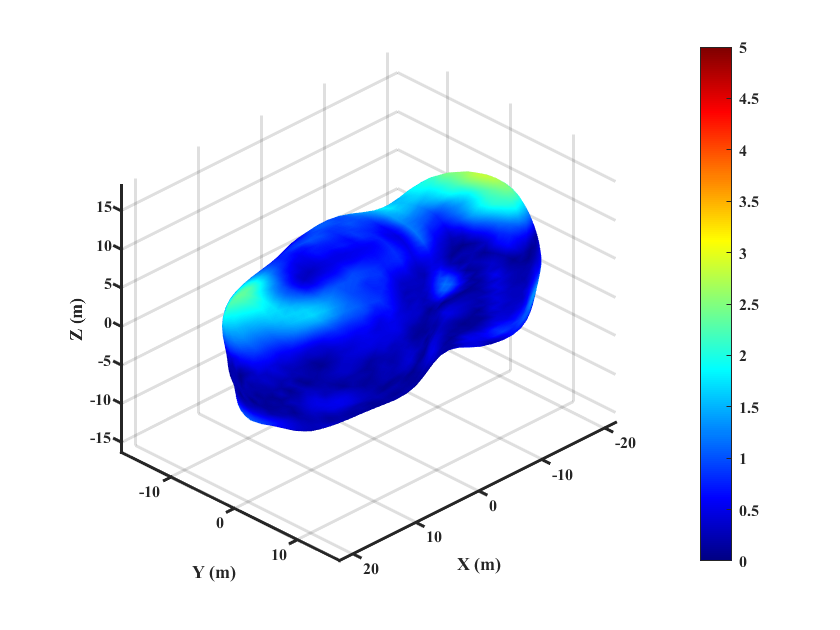
\includegraphics[width=0.6\columnwidth]{ErrorHeatmap.png}}
	\caption{3D surface error heatmap of the refined reconstruction model.}
	\label{fig_error_heatmap}
\end{figure}

Although a minor $0.81$-m contraction occurs along the Z-axis, this anisotropic performance mathematically reflects the highly heterogeneous exposure distribution. In low-exposure polar regions with severe grazing angles, as illustrated in Fig.~\ref{fig_exposure_heatmap}, the adaptive weight prioritizes Laplacian regularization to suppress thermal noise. This physically consistent tradeoff—sacrificing minor polar volume for global topological stability—ultimately ensures the robust 76.41\% F-score and morphologically consistent ISAR projections, as shown in the third and sixth rows of Fig.\ref{fig_disp_full_width}.

\begin{figure}[htbp]
	\centerline{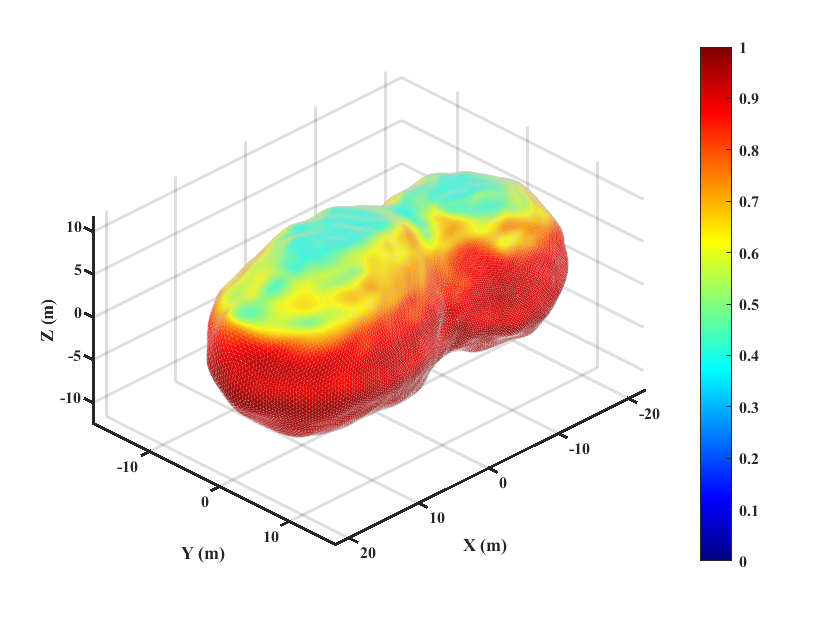
\includegraphics[width=0.6\columnwidth]{Exposure_Heatmap.png}}
	\caption{Cumulative radar exposure heatmap on the ground truth model.}
	\label{fig_exposure_heatmap}
\end{figure}

\section{Conclusion}\label{sec_five}
This paper presents a characterization framework for non-cooperative asteroids using ground-based ISAR observations. To overcome the geometric coupling between rotation parameters and absolute scale, a rotation estimation strategy based on dynamic envelope consistency is proposed. By matching the temporal evolution trends of geometric envelopes and utilizing the Pearson Correlation Coefficient, the rotation dynamics are effectively decoupled from the target’s absolute dimensions. Furthermore, a two-stage shape inversion method is employed to recover the 3D morphology by transforming the high-dimensional vertex optimization into a 1D scalar displacement problem along analytical surface normals. Simulation results based on the 1999~JV6 model and 1999~AN10 ephemeris validate the effectiveness of the proposed framework. Future work will focus on the processing of real-world observation data.

\section*{Acknowledgment}

The authors would like to acknowledge the JPL for providing the asteroid ephemeris data used in this study. Furthermore, we extend our gratitude to the 3D Asteroid Catalogue for providing the 3D asteroid shape models, which were instrumental in the ISAR imaging simulation and 3D reconstruction experiments.


\bibliographystyle{IEEEtran}
\bibliography{CIE}
\end{document}
